\section{Online Algorithm}
\label{sec:policy}

\looseness=-1
PACE's online compilation algorithm uses observed task arrivals and compilation outcomes to make cost-aware compilation proposals, with a separate cumulative budget to limit spending.
The proposal can be wrong about future arrivals or verification, while the budget uses only arrivals already observed and costs already charged.
The algorithm serves the current task before considering compilation for later tasks.

\begin{figure}[tbp]
\vspace{-5pt}% Trim excess space above this in-text figure.
\centering
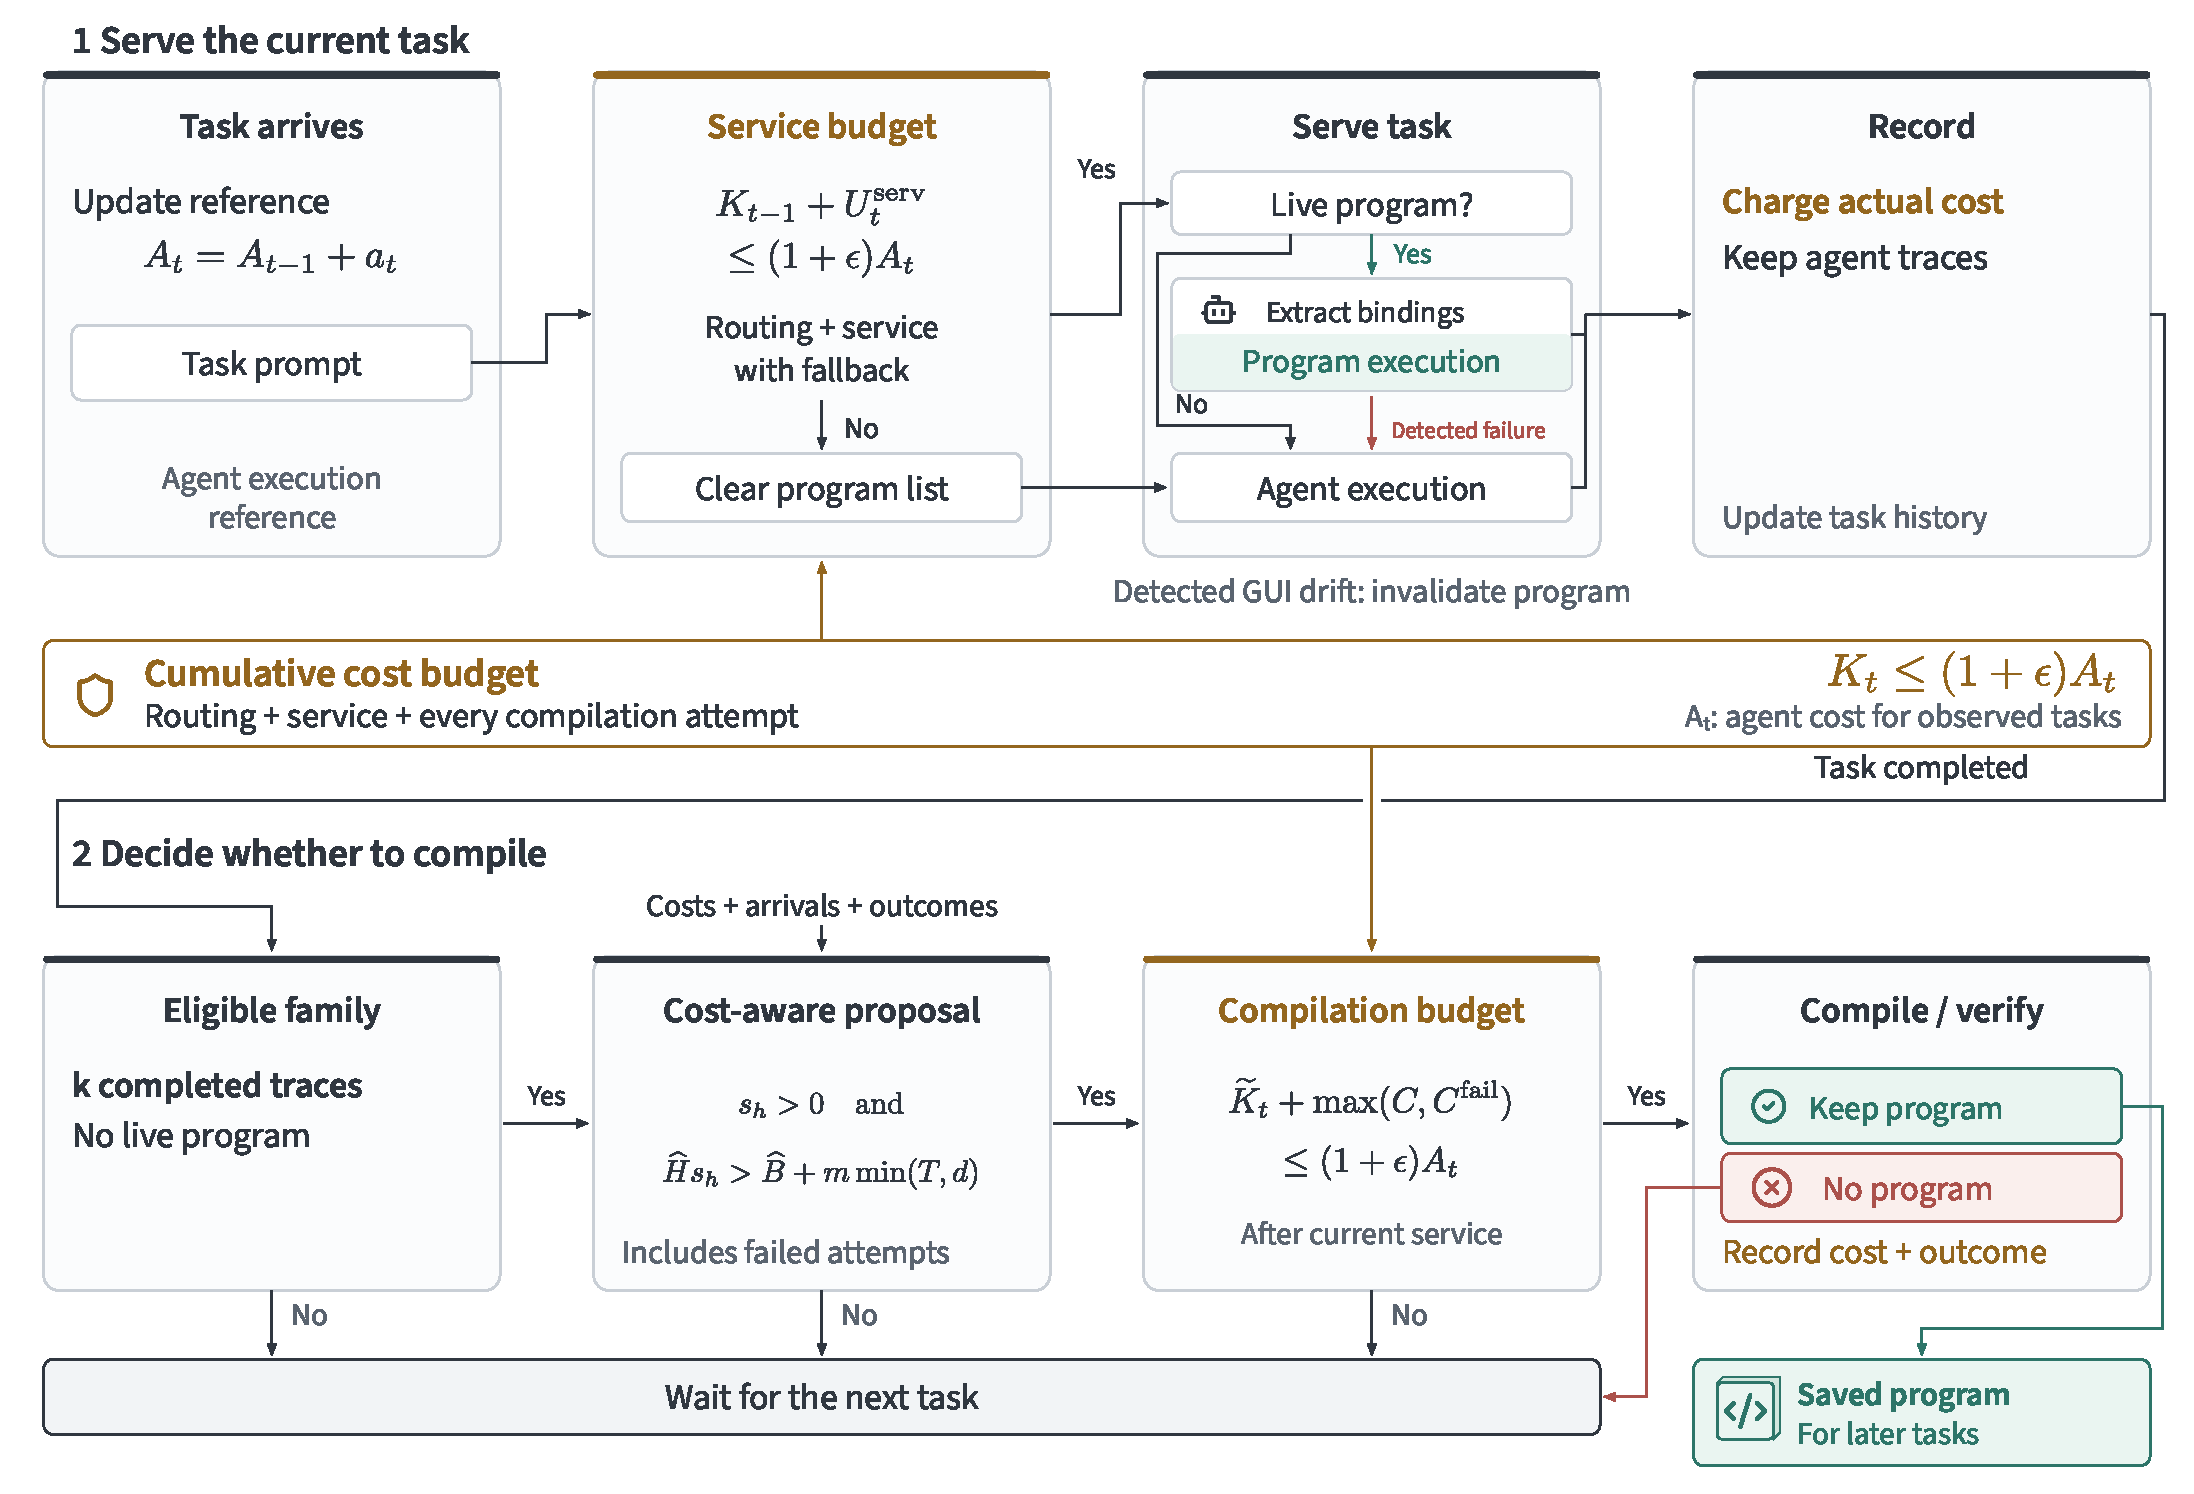
\includegraphics[width=\linewidth]{fig/online_algorithm_iclr27.pdf}
\caption{\looseness=-1 PACE's online compilation algorithm.
After serving a task, PACE checks trace availability, estimated savings, and the cost budget before compiling.
A failed check leads to waiting, while successful verification adds a program for later tasks.
The two budget checks use the same cumulative cost budget.}
\label{fig:online-algorithm}
\vspace{-6pt}% Preserve the template caption gap and at least a line below.
\end{figure}

\subsection{Cost-aware compilation proposal}
\label{sec:fullpolicy}

A family has enough traces for compilation after $k$ completed agent runs, including fallbacks.
Let $N$ be the number of arrivals observed for this family.
Let $d=t-t_{\mathrm{first}}$, where $t_{\mathrm{first}}$ is the index of its first arrival in the full task stream.
Thus $d=0$ on the family's first arrival.
After $j$ compilation attempts and $g$ successful verifications, define
\begin{equation}
\hat H=\min\!\left(\frac{Nd}{d+5},\frac1h\right),\qquad
\hat p=\frac{g+1}{j+2},\qquad
\hat B=C+\left(\frac1{\hat p}-1\right)C^{\mathrm{fail}}.
\label{eq:estimated-compile-cost}
\end{equation}
\looseness=-1
We use $1/0=\infty$.
This count estimates future reuse, with the mean program lifetime defined by $h$ as its upper limit.
We compute it from observed arrivals without training a prediction model.
The estimated compilation cost $\hat B$ includes failed attempts before verification succeeds, under the independent-retry interpretation derived in Appendix~\ref{app:reference}.
The cost guarantee does not require an accurate reuse estimate or independent retry outcomes.

With drift-adjusted saving $s_h=c-c^{\mathrm{prog}}-[h+(1-h)q]c$, a family with enough traces and no program to reuse proposes compilation when
\begin{equation}
s_h>0\quad\text{and}\quad\hat Hs_h>\hat B+m\min(T,d).
\label{eq:trigger}
\end{equation}
\looseness=-1
We call this condition the savings test.
The final term estimates the routing cost while one program remains on the list.
PACE removes entries after $T$ arrivals without use but keeps the programs.
It can add a program to the list again unless GUI drift has made it stop working.
The proposal accounts for the two sources of uncertain payback separately.
Low verification probability increases the estimated number of paid failures before producing a program, whereas GUI drift reduces the estimated reuse count after verification.
An expensive failed attempt can therefore make compilation unattractive even when successful construction is cheap.
The following budget checks limit the cost when these estimates are wrong.
Appendix~\ref{sec:matched-budget} compares alternative proposals with the same budget.
Their similar costs do not identify the exact estimators in Equation~\ref{eq:estimated-compile-cost} as a separate contribution.

\subsection{Budget checks}
\label{sec:budget-checks}

Before routing, PACE removes idle entries and adds any saved program that can still be reused for the arriving family to the list.
The next budget check decides whether this list can be used.
The program list shows the model which programs are available for routing.
This routing cost is paid on every arrival, including tasks served by the agent.
Keeping a program costs no tokens, but leaving it on the list adds routing cost on later tasks.
For a list of $\ell_t$ programs, PACE reserves enough budget for the largest possible service charge:
\begin{equation}
U_t^{\mathrm{serv}}=\tau_0+m\ell_t+
\begin{cases}
c,&\text{agent service},\\
c^{\mathrm{prog}}+c,&\text{program service}.
\end{cases}
\label{eq:service-reserve}
\end{equation}
The program reservation includes a possible fallback.
Service proceeds only if $K_{t-1}+U_t^{\mathrm{serv}}\leq(1+\epsilon)A_t$.
Otherwise PACE clears the program list before routing and uses the agent, whose charge is at most $a_t$.
Clearing the list keeps the programs and does not require any future spending.

Let $\widetilde K_t$ be the cumulative charge after service.
A proposed compilation proceeds only if
\begin{equation}
\widetilde K_t+\max(C,C^{\mathrm{fail}})\leq(1+\epsilon)A_t.
\label{eq:compile-budget}
\end{equation}
PACE then adds the actual compilation charge to its cumulative cost, including failed attempts and any compilation after the last service.
Savings can fund compilation across families, but estimated future reuse adds no budget.
Appendix~\ref{app:protocol-details} gives the complete execution order.

\subsection{Cost guarantee}
\label{sec:guarantee}

\begin{theorem}[Cost bound relative to agent execution]
\label{thm:cost-bound}
Let the reference increments $a_t$ be nonnegative.
Suppose every proposed action has a known finite charge bound, and clearing the program list before routing costs no tokens, requires no future spending, and allows default service at cost at most $a_t$.
For any $\epsilon\geq0$, PACE with exact arithmetic and valid reservations satisfies
\begin{equation}
K_t\leq(1+\epsilon)A_t
\quad\text{after each arrival }t
\label{eq:cost-guarantee}
\end{equation}
on every history allowed by these charge bounds.
\end{theorem}

\begin{proof}
The bound holds after both steps.
If service passes the budget check, its cost is at most the reserved amount.
If the check fails, default service adds at most $a_t$, so
\[
K_{t-1}+a_t\leq(1+\epsilon)A_{t-1}+a_t\leq(1+\epsilon)A_t.
\]
The compilation check keeps the same bound for either outcome.
Starting from $K_0=A_0=0$ establishes the result by induction.
\end{proof}

\looseness=-1
The fixed-charge model satisfies the assumptions with $a_t=\tau_0+c$.
The implementation permits tolerance $10^{-8}\max\{1,(1+\epsilon)A_t\}$.
The bound is global over the stream and concerns cost, not task errors or per-family spending.
When actual costs vary, spending must stay within the reserved amounts, and default service must cost at most $a_t$.
Historical means alone do not ensure these conditions.
PACE satisfies the cost constraint in Equation~\ref{eq:objective}, but we do not claim that it minimizes expected cost.
